\chapter{Analisi dei dati di ALICE} \label{Analisi}


\section{I Dati Iniziali}

I dati utilizzati per l'analisi svolta sono relativi a collisioni di due fasci di protoni incidenti al Cern. I dati, racccolti nel 2017 da ALICE, sono caratterizzati da un valore di energia nel centro di massa di 5 \ $TeV$. 
\\Da questi dati si vogliono selezionare solo le $D^{*+}$, che sono state ricostruite dal decadimento $D^{*+} \rightarrow D^0 + \pi^+ $. Per fare ciò, ai dati utilizzati sono già state applicate delle pre-selezioni estremamente morbide che permettono di preservare tutto il segnale e di fare una prima scrematura dei dati grezzi.
Gli intervalli di $p_T$ considerati sono: [1,2], [2,3], [3,4], [4,5], [5,6], [6,8], [8,12] misurati in GeV/c. 
La distribuzione di massa invariante iniziale, cioè prima dell'applicazione del BDT, è visibile in figura \ref{fig:grafmassDstar1} per l'intervallo di $p_T$ [2,3] $GeV/c$.

    \begin{figure}[htbp]
        \centering
        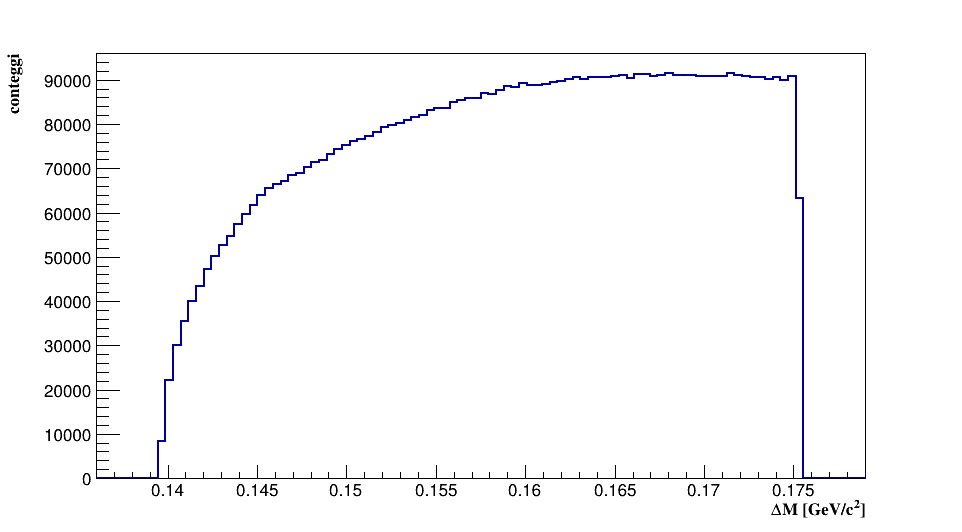
\includegraphics[width=0.7\linewidth]{AnalisiDati/dati_2_3.png}
        \caption{Distribuzione della differenza di massa invariante tra la $D^{*+}$ e la $D^0$, $\Delta M = M(\pi^+,\pi^+,K^-) - M(\pi^+,K^-)$, per l'intervallo di $p_T$ [2,3] $GeV/c$}
        \label{fig:grafmassDstar1}
    \end{figure}
    
Nel grafico \ref{fig:grafmassDstar1} non si vede nessun picco evidente, cosa che ci si aspetta nel caso di una risonanza come la $D^{*+}$. Questo accade perché il numero di $D^{*+}$ prodotte è troppo piccolo rispetto al fondo combinatoriale delle combinazioni di particelle non relative alla $D^{*+}$ e pertanto il picco della $D^{*+}$ non è riconoscibile rispetto al fondo.

    \begin{figure}[htbp]
        \centering
        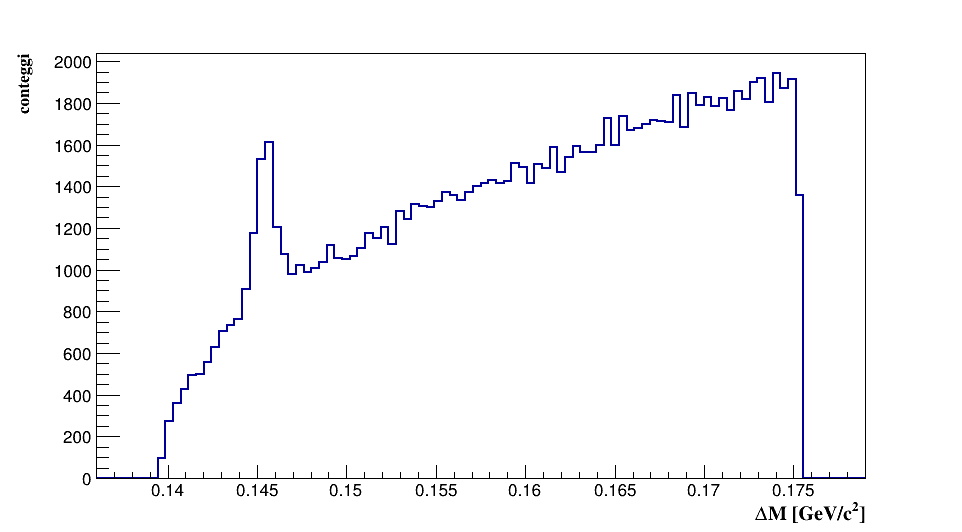
\includegraphics[width=0.7\linewidth]{AnalisiDati/dati_6_8.png}
        \caption{Distribuzione della differenza di massa invariante tra la $D^{*+}$ e la $D^0$, $\Delta M = M(\pi^+,\pi^+,K^-) - M(\pi^+,K^-)$, per l'intervallo di $p_T$ [6,8] GeV/c}
        \label{fig:grafmassDstar2}
    \end{figure}

Nel grafico della distribuzione di massa invariante \ref{fig:grafmassDstar2} in cui si considera l'intervallo di $p_T$ [6,8] GeV/c il picco della $D^{*+}$ è visibile e riconoscibile rispetto al fondo. 
\\In generale all'aumentare del valore del $p_T$ diventa più evidente il picco di segnale nelle distribuzioni di massa invariante. Questo accade perché nelle collisioni pp vengono prodotti più $\pi^+$ e $K^-$ con basso $p_T$ che con alto $p_T$ e perciò anche il fondo combinatoriale è maggiore a basso $p_T$.


\section{Applicazione del BDT}
Una volta finite le fasi di training e testing si può procedere all'applicazione del BDT sui dati che si vogliono analizzare. La struttura del BDT creata nella fase di training e  controllata nella fase del testing viene ora utilizzata per discriminare i dati tra segnale e fondo. Pertanto il BDT con 300 alberi, profondità massima 3 e con i valori di taglio indicati nella tabella \ref{Tab:tagli} è stato applicato per ogni intervallo di $p_T$ considerato, ottenendo così una selezione dei dati.
\\In figura \ref{fig:diffDstarD0_3_4_BDT} è riportata la distribuzione in massa invariante delle candidate $D^{*+}$ selezionate con il metodo BDT. Si vede il picco del segnale evidente attorno al valore della $ \Delta M = M(\pi^+,\pi^+,K^-) - M(\pi^+,K^-) \ \simeq \ 0.145 \ GeV/c$, sovrapposto ad un fondo residuo.


 \begin{figure}[htbp] 
        \centering
        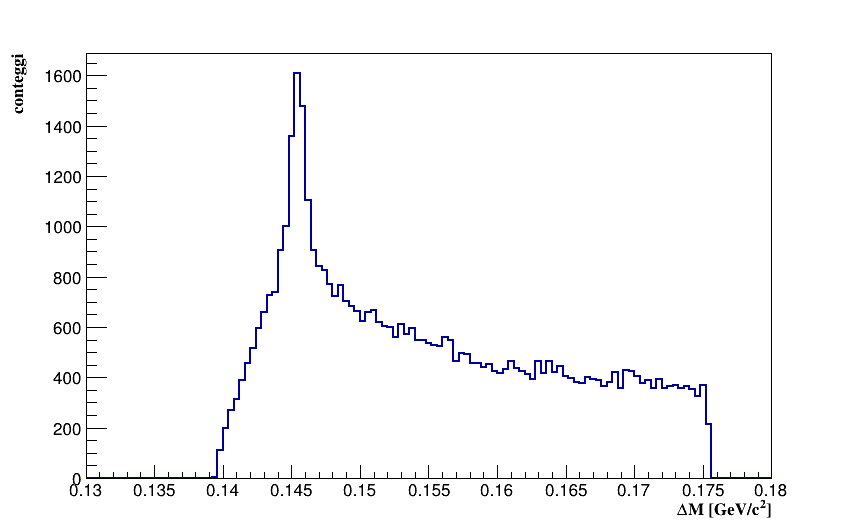
\includegraphics[width=0.7\linewidth]{AnalisiDati/diffDstarD0_3_4BDT.png}
        \caption{Distribuzione di massa invariante $\Delta M = M(\pi^+,\pi^+,K^-) - M(\pi^+,K^-)$, per l'intervallo di $p_T$ [3,4] GeV/c}
        \label{fig:diffDstarD0_3_4_BDT}
    \end{figure}
    
Per determinare il numero di candidate $D^{*+}$ selezionate si è proceduto con il fit della distribuzione di massa invariante. 
\\Per l'intervallo di $p_T$ [1-2] $GeV/c$ i dati della distribuzione di massa invariante delle candidate $D^{*+}$ selezionate con il metodo BDT non mostra un picco di segnale. Per questo motivo si è deciso di non procedere con il fit della distribuzione per questo intervallo di $p_T$ e perciò i risultati seguenti vengono mostrati solo per $p_T > 2 \ GeV/c$.
\\Per gli intervalli di $p-T$ considerati il picco del segnale é stato descritto da una funzione Gaussiana, mentre il fondo é stato descritto dalla somma di due funzioni:

    \begin{equation}
        fondo_1  = \ d \sqrt{x-0.13957} e^{- (x - 0.13857) }
    \end{equation}
     \begin{equation}
        fondo_2 = \ a x^2 + b x + c
    \end{equation}
    
Dove $a, \ b, \ c, e d$ sono dei parametri liberi utilizzati per il fit del fondo.
\\La $Gaussiana$ ha come range [0.144,0.147] , la funzione $fondo_1$ [0.1395,0.155] e $fondo_2$  [0.1435,0.150]. Le due funzioni per il fondo vengono prima sommate e poi la nuova funzione $fondo$ = $fondo_1$ + $fondo_2$ viene fatto il fit nell'intervallo [0.1395,0.1545]. Infine si sommano le funzione $fondo$ e $Gaussiana$ ottenendo la funzione chiamata $totale$, da cui il fit finale mostrato in figura \ref{fig:fit_3_4}.

    \begin{figure}[htbp] 
        \centering
        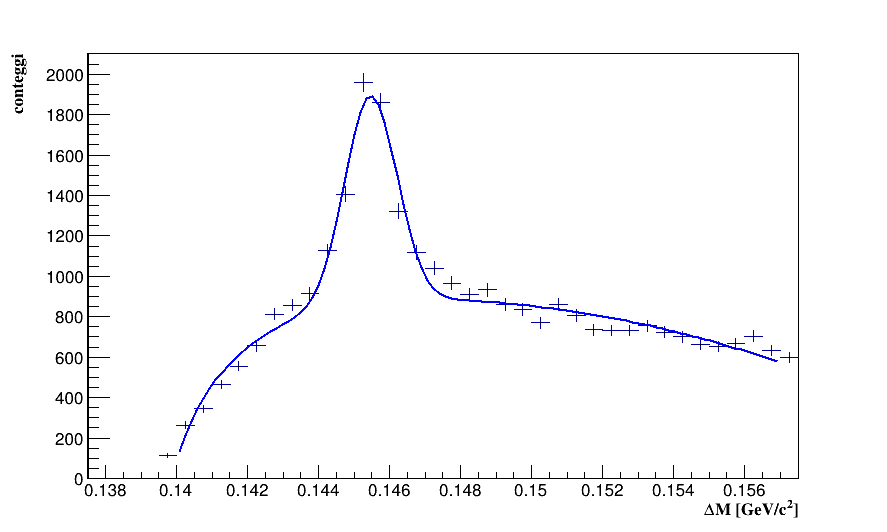
\includegraphics[width=0.9\linewidth]{AnalisiDati/pt_3_4_pol2.png}
        \caption{Distribuzione di massa invariante $\Delta M = M(\pi^+,\pi^+,K^-) - M(\pi^+,K^-)$, per l'intervallo di $p_T$ [3,4] GeV/c e funzione di fit $totale$ in blu}
        \label{fig:fit_3_4}
    \end{figure}
    
Si nota che all'aumentare del $p_T$ il fondo diminuisce sempre di più e tende ad appiattirsi, rendendo così il fit più semplice.
Si riportano di seguito i grafici per i vari bin di $p_T$ considerati. 
\\

\begin{minipage}{.5\textwidth}%{0.5 cm} 
        \begin{flushleft} \large
        \flushleft
        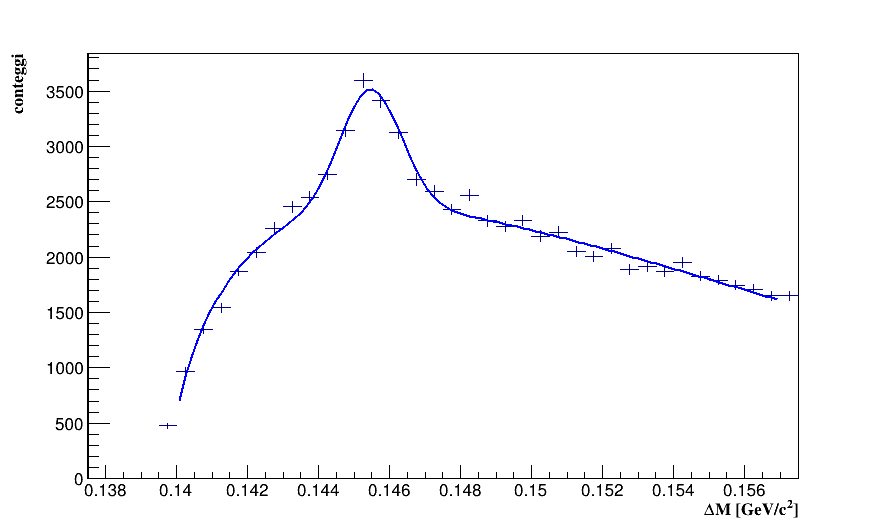
\includegraphics[width=8cm]{AnalisiDati/pt_2_3_pol2.png}
        \captionof{figure}{Distribuzione di massa invariante $\Delta M = M(\pi^+,\pi^+,K^-) - M(\pi^+,K^-)$, per l'intervallo di $p_T$ [2,3] GeV/c e funzione di fit $totale$ in blu}
        \label{fig:fit_2_3}
        \end{flushleft}
        \end{minipage}
    ~
    \begin{minipage}{0.5\textwidth}
        \begin{flushright} \large
        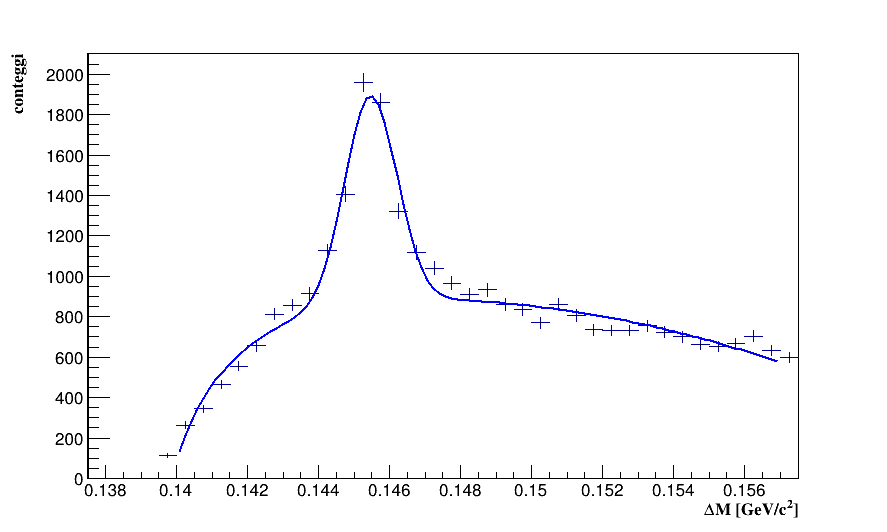
\includegraphics[width=8cm]{AnalisiDati/pt_3_4_pol2.png}
        \captionof{figure}{Distribuzione di massa invariante $\Delta M = M(\pi^+,\pi^+,K^-) - M(\pi^+,K^-)$, per l'intervallo di $p_T$ [3,4] GeV/c e funzione di fit $totale$ in blu}
        \label{fig:fit_3_4_p}
        \end{flushright}
    \end{minipage} \\[1.cm]
    
    
    \begin{minipage}{.5\textwidth}%{0.5 cm} 
        \begin{flushleft} \large
        \flushleft
        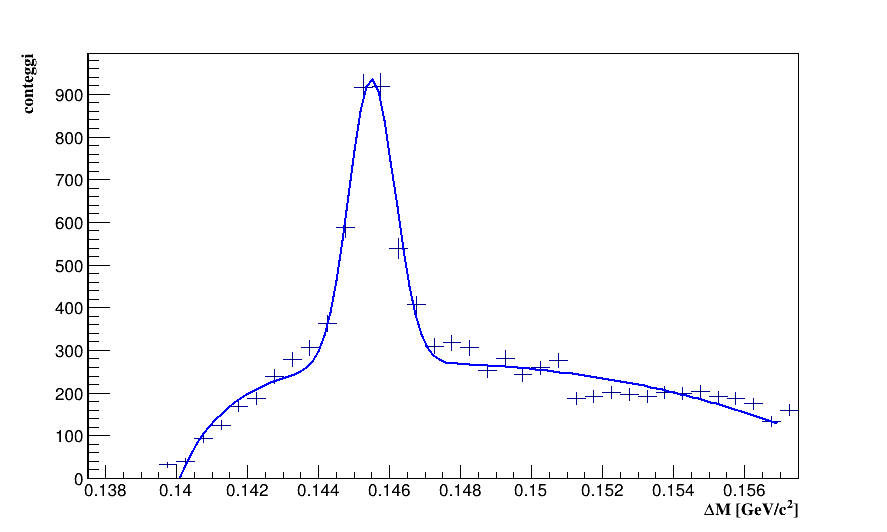
\includegraphics[width=8cm]{AnalisiDati/pt_4_5_pol2.png}
        \captionof{figure}{Distribuzione di massa invariante $\Delta M = M(\pi^+,\pi^+,K^-) - M(\pi^+,K^-)$, per l'intervallo di $p_T$ [4,5] GeV/c e funzione di fit $totale$ in blu}
        \label{fig:fit_4_5}
        \end{flushleft}
        \end{minipage}
    ~
    \begin{minipage}{0.5\textwidth}
        \begin{flushright} \large
        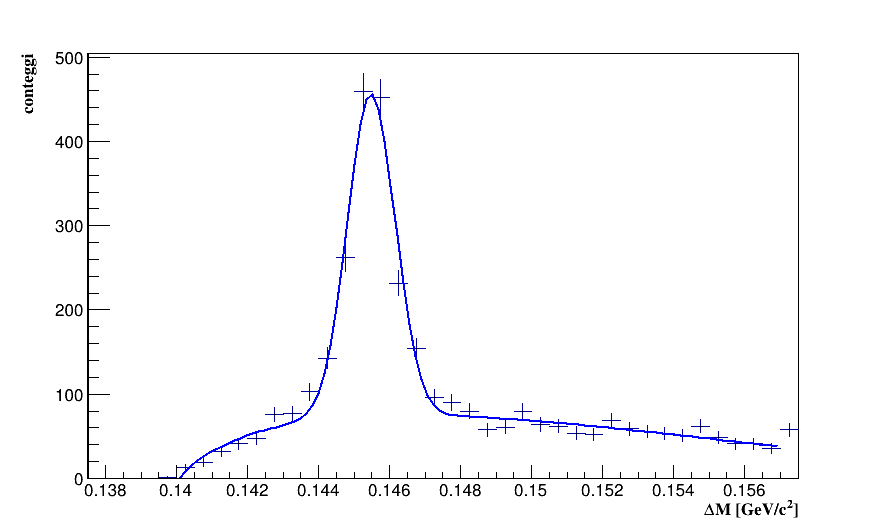
\includegraphics[width=8cm]{AnalisiDati/pt_5_6_pol2.png}
        \captionof{figure}{Distribuzione di massa invariante $\Delta M = M(\pi^+,\pi^+,K^-) - M(\pi^+,K^-)$, per l'intervallo di $p_T$ [5,6] GeV/c e funzione di fit $totale$ in blu}
        \label{fig:fit_5_6}
        \end{flushright}
    \end{minipage} \\[1.cm]

\begin{minipage}{.5\textwidth}%{0.5 cm} 
        \begin{flushleft} \large
        \flushleft
        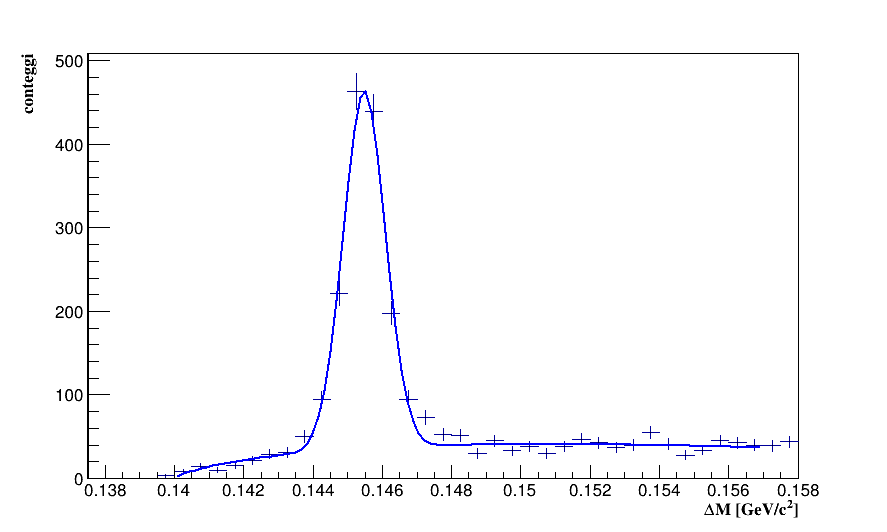
\includegraphics[width=8cm]{AnalisiDati/pt_6_8_pol2.png}
        \captionof{figure}{Distribuzione di massa invariante $\Delta M = M(\pi^+,\pi^+,K^-) - M(\pi^+,K^-)$, per l'intervallo di $p_T$ [6,8] GeV/c e funzione di fit $totale$ in blu}
        \label{fig:fit_6_8}
        \end{flushleft}
        \end{minipage}
    ~
    \begin{minipage}{0.5\textwidth}
        \begin{flushright} \large
        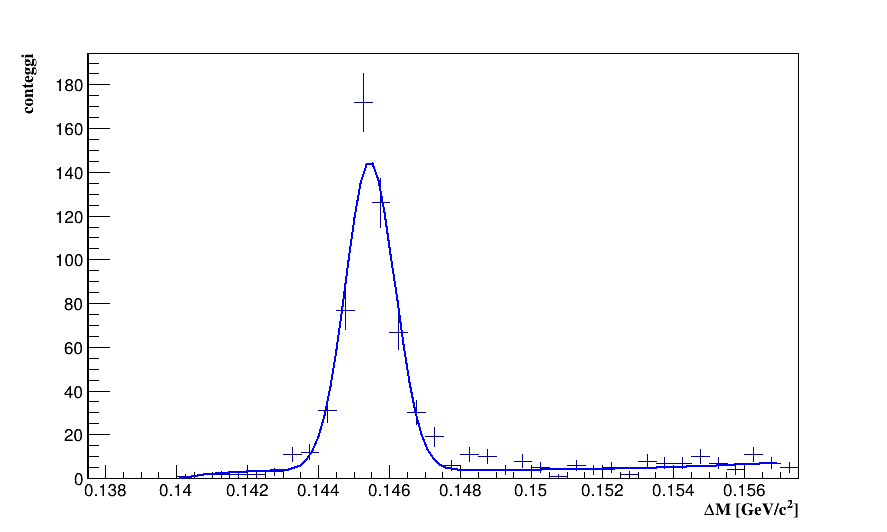
\includegraphics[width=8cm]{AnalisiDati/pt_8_12_pol2.png}
        \captionof{figure}{Distribuzione di massa invariante $\Delta M = M(\pi^+,\pi^+,K^-) - M(\pi^+,K^-)$, per l'intervallo di $p_T$ [8,12] GeV/c e funzione di fit $totale$ in blu}
        \label{fig:fit_8_12}
        \end{flushright}
    \end{minipage} \\[1.cm]
    


\section{Valutazione delle performance}

Per valutare le performance dell'analisi svolta si sono calcolate alcune grandezze quali la quantità di segnale selezionata, la quantità di fondo selezionata, la significatività e il rapporto segnale su fondo. Per poter avere queste grandezze in ogni intervallo di $p_T$ si è calcolato l'integrale della funzione di fit $totale$ entro 3 $\sigma$ a destra e a sinistra del valore medio della Gaussiana. Sia il valore medio della Gaussiana che il valore della $\sigma$ sono stati presi dal fit della Gaussiana sul picco del segnale. Poi si è trovata la quantità di fondo calcolando l'integrale della funzione $fondo$ nello stesso intervallo. Infine, per trovare la quantità di segnale, si è sottratto all'integrale della funzione $totale$ l'integrale del fondo. 
\\In figura \ref{fig:segnale} si riporta la quantità di segnale per i vari intervalli di $p_T$ con l'errore associato. Dalla figura si vede che l'efficienza del segnale diminuisce all'aumentare del $p_T$.

    \begin{figure}[htbp] 
        \centering
        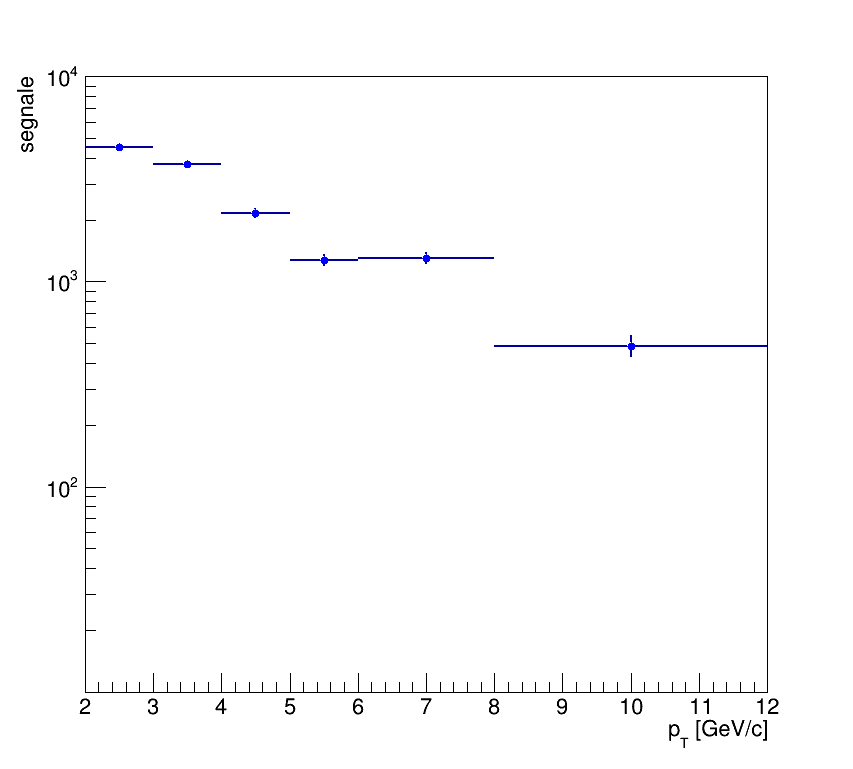
\includegraphics[width=0.9\linewidth]{AnalisiDati/segnale.png}
        \caption{Grafico della quantità di segnale in funzione del $p_T$}
        \label{fig:segnale}
    \end{figure}

In figura \ref{fig:fondo} è mostrata la quantità di fondo per gli intervalli di $p_T$ considerati. Si vede che l'efficienza del segnale diminuisce velocemente all'aumentare del $p_T$.

    \begin{figure}[htbp] 
        \centering
        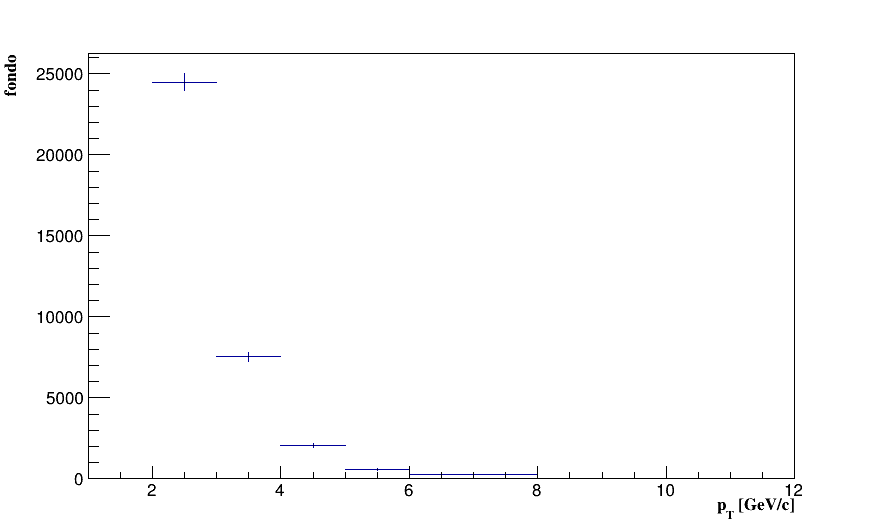
\includegraphics[width=0.9\linewidth]{AnalisiDati/fondo.png}
        \caption{Grafico della quantità di fondo in funzione del $p_T$}
        \label{fig:fondo}
    \end{figure}
    
Si è calcolata anche la significatività, utilizzando la formula 
 
 \begin{equation}
     sign = \frac{s}{\sqrt{s+f}}
 \end{equation}

dove $s$ è la quantità di segnale, mentre $f$ è la quantità di fondo. Anche in questo caso l'operazione è stata ripetuta per tutti gli intervalli di $p_T$ e con la propagazione degli errori si è ricavato l'errore relativo.

    \begin{figure}[htbp] 
        \centering
        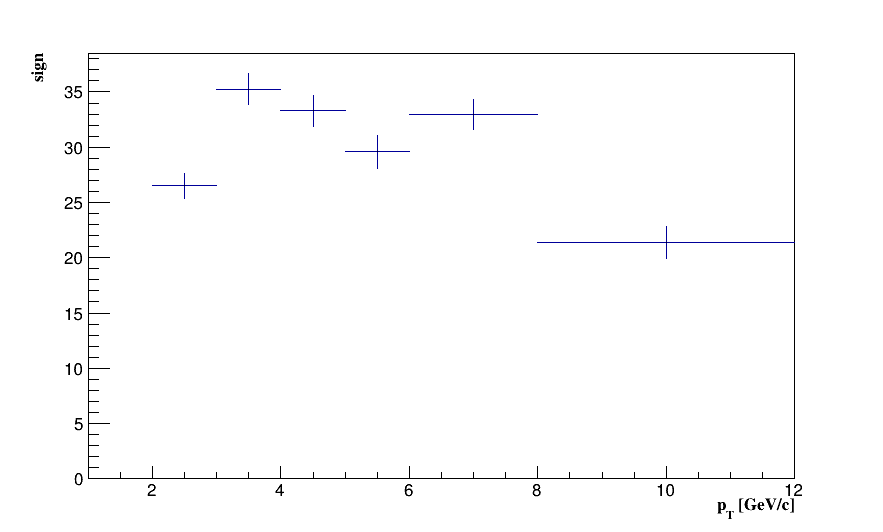
\includegraphics[width=0.9\linewidth]{AnalisiDati/significance.png}
        \caption{Grafico della significatività in funzione del $p_T$}
        \label{fig:significatività}
    \end{figure}

Il grafico in figura \ref{fig:significatività} mostra il valore della significatività per gli intervalli di $p_T$ considerati. Si vede che si ha il massimo della significatività per l'intervallo di $p_T$ [3,4] GeV/c e il minimo per l'intervallo di $p_T$ [8,12] GeV/c.
\\Si è creato anche il grafico del rapporto tra segnale e fondo al variare del bin di $p_T$ riportato in figura \ref{fig:s_b}. 

    \begin{figure}[htbp] 
        \centering
        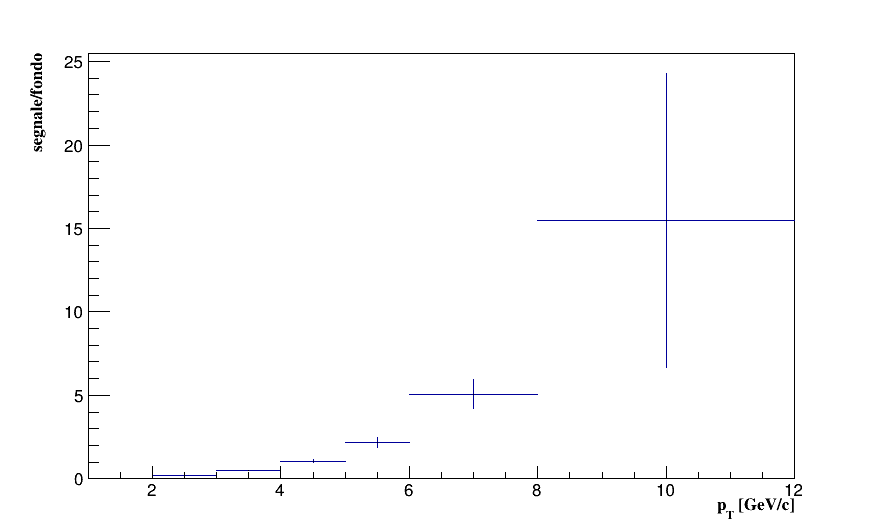
\includegraphics[width=0.9\linewidth]{AnalisiDati/s_b.png}
        \caption{Grafico del rapporto segnale su fondo in funzione del $p_T$}
        \label{fig:s_b}
    \end{figure}
    
Infine, in figura \ref{fig:confr_sign}, si confrontano i valori della significatività ottenuti con l'analisi del BDT e quelli ottenuti con l'analisi standard si ALICE. Si vede che per gli intervalli di $p_T < 4 \ GeV/c$ la significatività ottenuta con l'analisi del BDT è più alta di quella ottenuta con l'analisi standard di ALICE, mentre per $p_T > 4 \ GeV/c$ accade il contrario. 

\begin{figure}[htbp] 
        \centering
        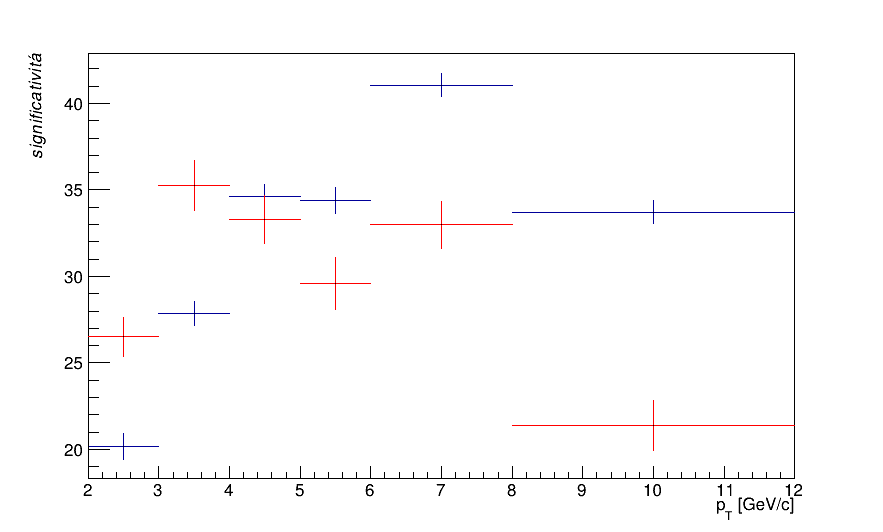
\includegraphics[width=0.9\linewidth]{AnalisiDati/confr_sign.png}
        \caption{Grafico della significatività in funzione del $p_T$, in blu l'analisi standard di ALICE, in rosso l'analisi con il BDT}
        \label{fig:confr_sign}
    \end{figure}
